% draft.tex does not \input this file; kept because it holds material not copied into appendix.tex
\section{Latency and Cost}
\label{sec:latency}

We account for provider spend and end-to-end latency on the full evaluation pack using list prices recorded on 2026-10-19 in the study configuration.
Charges sum logged token and text-unit usage from harness runs, new full-pack API calls, and development-pool scoring; cache-only metric rebands add no marginal cost.
Table~\ref{tab:spend} itemizes the billable components that total \$18.38 for this study.

\begin{table}[t]
  \centering
  \caption{Provider spend (USD) for run \texttt{20261020T040920Z\_90c5fd13}.}
  \label{tab:spend}
  \begin{tabular}{lr}
    \toprule
    Charge component & USD \\
    \midrule
    Jev harness (7{,}138{,}858 input tokens) & 0.2998 \\
    Full-pack new calls, Jev & 0.1091 \\
    Full-pack new calls, Clef & 4.7130 \\
    Full-pack new calls, Clef-flash & 0.7464 \\
    Full-pack new calls, Guardrails (24{,}391 text units) & 3.6586 \\
    Development-pool scoring & 8.8542 \\
    Step 3 smoke, logged token charges & 0.0027 \\
    Metrics reband and rerun (cache only) & 0.00 \\
    \midrule
    Total & 18.38 \\
    \bottomrule
  \end{tabular}
\end{table}

Development-pool scoring is the largest line item because threshold and cascade tuning scored every arm on held-out development rows before the reported test metrics.
Guardrails full-pack cost reflects per-text-unit Bedrock pricing on tens of thousands of assessments, while Jev full-pack new calls remain a small fraction of total spend after the harness validation run.

Normalized to one thousand scored prompts on the full pack, average cost is \$0.023 for Jev, \$0.230 for Clef, \$0.036 for Clef-flash, and \$0.179 for Guardrails.\footnote{Full-precision JSON: Jev \texttt{cost\_per\_1000\_prompts\_usd} = 0.02320827919921875; Clef = 0.2301770390625; Clef-flash = 0.036452848925781246; Guardrails = 0.17864501953125.}
Jev is an order of magnitude cheaper per prompt than Clef and several times cheaper than Guardrails on this pack, with Clef-flash between Jev and Guardrails on cost.

Latency is taken from each row's stored \texttt{latency\_ms} on the original provider call.
Rows replayed from cache retain that recorded latency rather than reporting a near-zero cache read time, so medians reflect the API latency distribution of the underlying requests.
For Jev the median is 88.9\,ms across all full-pack rows, with a live-call-only median of 88.0\,ms and p95 of 291\,ms when cache hits are excluded where identifiable.\footnote{JSON \texttt{median\_latency\_ms} = 88.86603199971432; \texttt{live\_call\_only\_median\_latency\_ms} = 88.02840700082015; \texttt{live\_call\_only\_p95\_latency\_ms} = 290.63895900071657.}
Clef median latency is 368\,ms, Clef-flash is 303\,ms, and Guardrails is 359\,ms.
Jev is the fastest arm by a wide margin in this region, while Clef and Guardrails cluster near 350 to 370\,ms medians.

Figure~\ref{fig:latency} places cost per thousand prompts against harmful miss rate on benchmarks where miss is defined, illustrating that cheaper arms are not uniformly safer.
The scatter connects economic choice to the safety metrics reported elsewhere in the paper rather than proposing a production budget.

\begin{figure}[t]
  \centering
  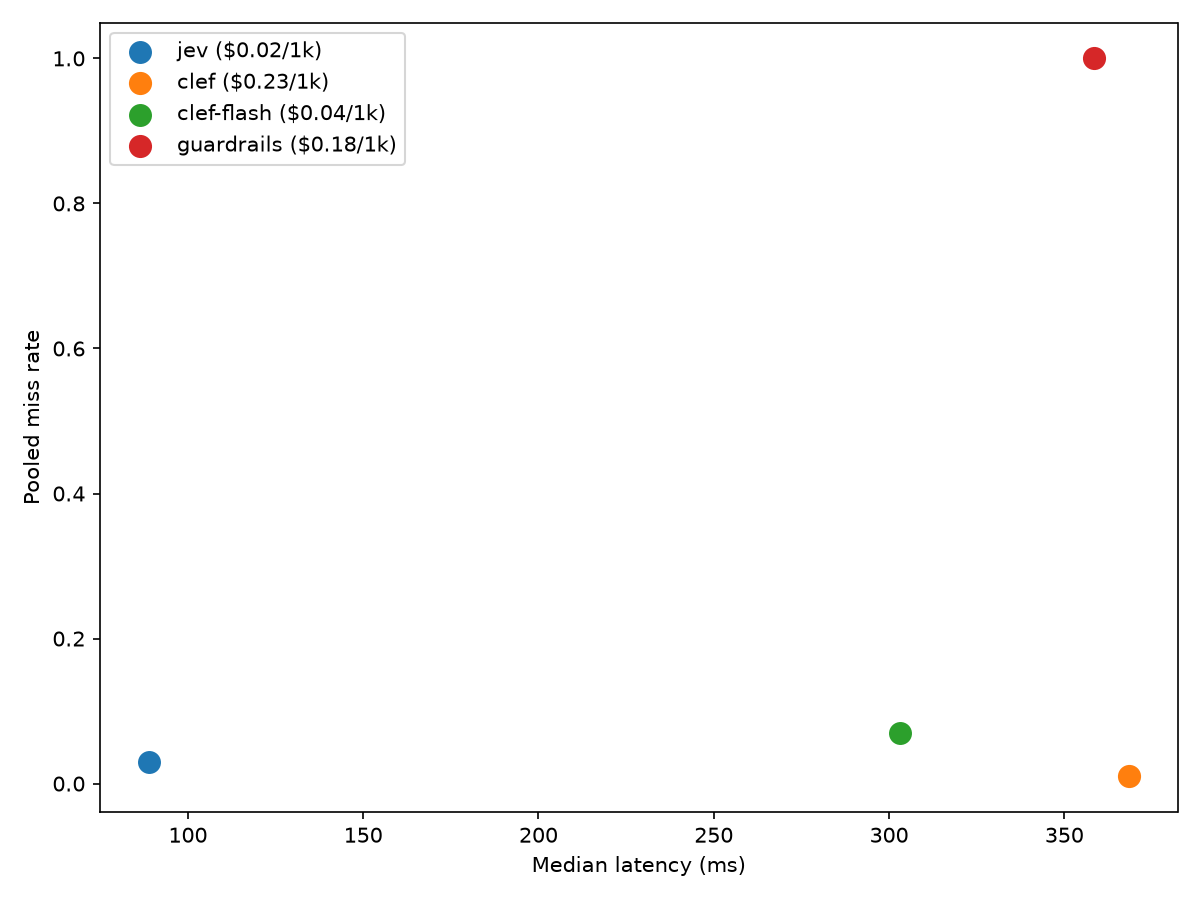
\includegraphics[width=\linewidth]{../outputs/figures/20261020T040920Z_90c5fd13/latency_cost_vs_miss.png}
  \caption{Cost per 1{,}000 prompts versus miss rate by arm and dataset.}
  \label{fig:latency}
\end{figure}

Interpreting latency and cost together, a product that screens every user turn with Clef plus Guardrails would pay roughly the sum of per-arm marginal costs on each prompt that runs both services, whereas Jev's sub-100\,ms median makes it viable as a first-stage filter before a managed guardrail.
Our stack experiments reuse saved predictions, so they do not add further latency charges beyond the arms already scored.
Reported dollars cover this benchmark matrix only and do not extrapolate to proprietary traffic volumes or reserved-capacity pricing.
